\documentclass[11pt, a4paper]{book}
\usepackage{./macros/jpA4}
\usepackage{./macros/BScMac}
\usepackage{./macros/BScTitel}
%% copyleft by Martin Schlather 2015

%%%%%%%%%%%%%%%%%%%%%%%%%%%%%%%%%%%%%%%%%%%%%%%%%%%%%%%%%%%%%%%%%%%%%%%%%%
%%% the command \fverbatim{filename} is able to plot most files without
%%% interpreting potential LaTeX-commands, so \fverbatim is the file
%%% version of \verbatim.
%%% Options: line numbering, just put the command \numbering in front.
%%%          the style used in the numbering can be redefined, using
%%%              \def\numstyle{\tt } e.g.            
%%%          the style for the text can be redefined using
%%%              \def\vstyle{\small }, e.g..              
%%%          the space between the numbers and the text can be
%%%              redefined using \def\vspaces{\ \ e.g.}.
%%% Good luck, Martin
\def\makeatletter{\catcode`\@=11\relax}
\def\makeatother{\catcode`\@=12\relax}
\makeatletter

%%%%% end notes, see LaTex-Tips, J.K. Shultis,
%%%%% \endnote,\printnotes
\newbox\endnotebox %author Erica M. S. Harris (modified by J. K. Shultis
\def\endnotesize{\footnotesize}
\newcounter{endnotecount}
\def\endnote{\stepcounter{endnotecount}%
          \xdef\@theenmark{[\theendnotecount]}\@endnotemark\@endnotetext}%
\def\@endnotemark{\leavevmode\ifhmode\edef\@x@sf{\the\spacefactor}\fi%
                  \hbox{$^{\@theenmark}$}%
          \ifhmode\spacefactor\@x@sf\fi\relax}%
\long\def\@endnotetext#1{\global\setbox\endnotebox=%
   \vbox{\hsize\columnwidth\@parboxrestore%
   \def\baselinestretch{1}\@normalsize%
   \unvbox\endnotebox\@makeentext{\ignorespaces#1\strut\par}}}%
\long\def\@makeentext#1{\parindent 1em \noindent%
% \hbox to 1.8em{\hss\@theenmark.~}#1}  %% -- use for normalsize
  \hbox to 1.8em{\hss\small\@theenmark.~}\small#1}  %% -- use for normalsize
% \hbox to 1.8em{\hss\endnotesize\@theenmark.~}\endnotesize#1} %<<<
\def\printnotes{%
\ifvoid\endnotebox\else\bigskip\bigskip{\Large\bf Endnotes}\\
\unvbox\endnotebox\par\fi%
\setcounter{endnotecount}{0}}


% Definition of  \fverbatim{filename}
\newread\ps@stream\newif\ifnot@eof
\newwrite\@unused
\def\xps@typeout#1{{\let\protect\string\immediate\write\@unused{#1}}}
\newif\if@num\@numfalse\countdef\num@z=230\dimendef\num@b=230\dimendef\@breite=231
\long\def\xepsf@aux#1:.:{\if@num\hbox to \num@b{\hfill\numstyle\the\num@z\vspaces\hss}\advance\num@z by 1\fi\hbox to \@breite{\vstyle #1\hss}\\}

\def\numstyle{\it}
\def\vstyle{\tt}
\def\numbering{\@numtrue}
\def\vspaces{\/\ \ }
\newbox\num@box
\def\fverbatim#1{\mbox{}\openin\ps@stream=#1
\ifeof\ps@stream\xps@typeout{Fehler, Datei #1 nicht gefunden}\else
   {\not@eoftrue \chardef\other=12
    \def\do##1{\catcode`##1=\other}\dospecials \catcode`\ =10
    \if@num\num@z1
       \loop
          {\obeyspaces\read\ps@stream to \epsf@tmp}\ifeof\ps@stream\not@eoffalse\fi
          \advance\num@z by 1
       \ifnot@eof\repeat
       \closein\ps@stream
       \setbox\num@box=\hbox{\numstyle\the\num@z\vspaces}
       \num@b\wd\num@box\num@z1
       \@breite\textwidth\advance\@breite by -\num@b
    \fi\not@eoftrue\openin\ps@stream=#1
    \loop
       {\obeyspaces
        \read\ps@stream to \epsf@tmp\global\let\epsf@fileline\epsf@tmp}%
       \ifeof\ps@stream\not@eoffalse\else
       \expandafter\xepsf@aux\epsf@fileline:.:%
       \fi
   \ifnot@eof\repeat
   }\closein\ps@stream\fi}%
\makeatother

\usepackage[paper=a4paper,left=32mm,right=32mm,top=32mm,bottom=32mm]{geometry}
\usepackage{hyperref}
%% neu
\usepackage[utf8]{inputenc}
\usepackage{microtype}
\usepackage{lmodern}
\usepackage{enumitem}
%\usepackage{halloweenmath}
%\usepackage{MnSymbol}
\usepackage{fontawesome}
\usepackage{bclogo}
\usepackage{csquotes}
\usepackage{tikz}
\usepackage{mathtools}
\usepackage{media9}
\usepackage{pgfplots}

\usepackage{titletoc}
\usepackage{ifthen}
\usepackage{animate}
\usepackage{subfig}
\usepackage{xparse}
\usepackage{pgfplots}
\usetikzlibrary{arrows.meta}
\usetikzlibrary{calc}
\usepgfplotslibrary{fillbetween}


\parindent0mm
\einseitig
\pagenumbering{gobble}

\pgfmathdeclarefunction{gauss}{2}{%
	\pgfmathparse{1/(#2*sqrt(2*pi))*exp(-((x-#1)^2)/(2*#2^2))}%
}

\tikzset{
	declare function={
		normcdf(\x,\m,\s)=1/(1 + exp(-0.07056*((\x-\m)/\s)^3 - 1.5976*(\x-\m)/\s));
	}
}

\ExplSyntaxOn
\DeclareExpandableDocumentCommand \round { O{0} m }
{ \fp_eval:n { round(#2,#1) } }
\ExplSyntaxOff

\newcommand\symbolwithin[2]{%
	{\mathmakebox[\widthof{\ensuremath{{}#2{}}}][c]{{#1}}}}

\renewcommand{\labelitemii}{\labelitemi}
\renewcommand{\thesubsection}{(\Alph{subsection})\hspace{-1em} }
%\titleformat{\subsection}[]{}{\Alph}{\quad}

\makeatletter
\def\moverlay{\mathpalette\mov@rlay}
\def\mov@rlay#1#2{\leavevmode\vtop{%
		\baselineskip\z@skip \lineskiplimit-\maxdimen
		\ialign{\hfil$\m@th#1##$\hfil\cr#2\crcr}}}
\newcommand{\charfusion}[3][\mathord]{
	#1{\ifx#1\mathop\vphantom{#2}\fi
		\mathpalette\mov@rlay{#2\cr#3}
	}
	\ifx#1\mathop\expandafter\displaylimits\fi}
\makeatother

\newcommand{\cupdot}{\charfusion[\mathbin]{\cup}{\cdot}}
\newcommand{\bigcupdot}{\charfusion[\mathop]{\bigcup}{\cdot}}
\newcommand{\platz}{\relax}
\newcommand{\dint}{\, \mathrm{d}}


\newcounter{slideIndex}
\setcounter{slideIndex}{1}
\setcounter{chapter}{3}

\newcommand{\UniAnim}{
	\begin{tikzpicture}
	\pgfmathsetmacro{\b}{1 + 0.05*(\theslideIndex - 1)};	
	\pgfmathsetmacro{\hoehe}{1/(\b - 0.5)}
	\def\Gauss{}
	\begin{axis}[
	legend pos = north east,
	x = 1cm,
	y = 2cm,
	axis lines=middle,
	axis line style={-Stealth,thick},
	xmin=-.625,xmax=6,ymin=-.3125,ymax=2.25,
	xtick={-1,0,1,2,3,4,5},
	ytick={0,0.5,1,1.5,2},
	extra x ticks={5.5},
	extra y ticks={-0.25},
	extra x tick style={xticklabel=\empty},
	extra y tick style={yticklabel=\empty},
	%xticklabel=\empty,
	%yticklabel=\empty,
	xtick distance=1,
	ytick distance=1,
	xlabel=$t$,
	ylabel=$f(t)$,
	%title={Wonderful plot},
	minor tick num= 1,
	grid style={thin,densely dotted,black!20}]	
	%\addplot [name path = B, domain = -1:2, color = blue, smooth] {gauss(\erwartw,\variance)};\addlegendentry{$\mu = \erwartw, \sigma^2= \variance$};	
	\addplot[domain = 0.5:\b, color = blue, smooth] {\hoehe};
	\addplot[domain = -0.5:0.5, color = blue, smooth] {0};
	\addplot[domain = \b:6, color = blue, smooth] {0};	
	\addplot[dotted, blue] coordinates{(0.5,0) (0.5,\hoehe)};	
	\addplot[dotted, blue] coordinates{(\b,0) (\b,\hoehe)};
	\end{axis}	
	\end{tikzpicture}\stepcounter{slideIndex}
}

\newcommand{\cdfUni}{
	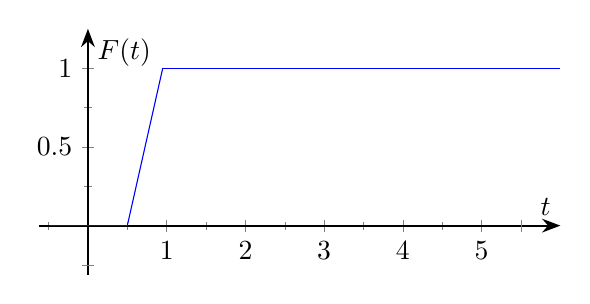
\begin{tikzpicture}
	\pgfmathsetmacro{\b}{1 + 0.05*(\theslideIndex - 1)};
	\def\Gauss{}
	\begin{axis}[
	legend pos = north east,
	x = 1cm,
	y = 2cm,
	axis lines=middle,
	axis line style={-Stealth,thick},
	xmin=-.625,xmax=6,ymin=-.3125,ymax=1.25,
	xtick={-1,0,1,2,3,4,5},
	ytick={0,0.5,1},
	extra x ticks={5.5},
	extra y ticks={-0.25},
	extra x tick style={xticklabel=\empty},
	extra y tick style={yticklabel=\empty},
	%xticklabel=\empty,
	%yticklabel=\empty,
	xtick distance=1,
	ytick distance=1,
	xlabel=$t$,
	ylabel=$F(t)$,
	%title={Wonderful plot},
	minor tick num= 1,
	grid style={thin,densely dotted,black!20}]	
	%\addplot [name path = B, domain = -1:2, color = blue, smooth] {gauss(\erwartw,\variance)};\addlegendentry{$\mu = \erwartw, \sigma^2= \variance$};	
	\addplot[domain = 0.5:\b, color = blue, smooth] {(x-0.5)/(\b - 0.5)};
	\addplot[domain = -0.5:0.5, color = blue, smooth] {0};
	\addplot[domain = \b:6, color = blue, smooth] {1};
	\end{axis}	
	\end{tikzpicture}\stepcounter{slideIndex}
}

\newcommand{\ExpAnim}{
	\begin{tikzpicture}
	\pgfmathsetmacro{\lambdaNeu}{\round[3]{0.25 + 0.025*(\theslideIndex - 2)} };
	\def\Gauss{}
	\begin{axis}[
	legend pos = north east,
	x = 1cm,
	y = 10cm,
	axis lines=middle,
	axis line style={-Stealth,thick},
	xmin=-.625,xmax=6,ymin=-0.0625,ymax=0.6,
	xtick={-1,0,1,2,3,4,5},
	ytick={0,0.1,0.2,0.3,0.4,0.5},
	extra x ticks={5.5},
	extra y ticks={-0.05,0.55},
	extra x tick style={xticklabel=\empty},
	extra y tick style={yticklabel=\empty},
	%xticklabel=\empty,
	%yticklabel=\empty,
	xtick distance=1,
	ytick distance=1,
	xlabel=$t$,
	ylabel=$f(t)$,
	%title={Wonderful plot},
	minor tick num= 1,
	grid style={thin,densely dotted,black!20}]	
	%\addplot [name path = B, domain = -1:2, color = blue, smooth] {gauss(\erwartw,\variance)};\addlegendentry{$\mu = \erwartw, \sigma^2= \variance$};	
	\addplot[domain = 0:6, color = blue, smooth] {\lambdaNeu*exp(-\lambdaNeu*x)};\addlegendentry{$\lambda = \lambdaNeu$};
	\addplot[domain = -0.5:0, color = blue, smooth] {0};
	\end{axis}	
	\end{tikzpicture}\stepcounter{slideIndex}
}

\newcommand{\cdfExp}{
	\begin{tikzpicture}
	\pgfmathsetmacro{\lambdaNeu}{\round[3]{0.25 + 0.025*(\theslideIndex - 2)} };
	\def\Gauss{}
	\begin{axis}[
	legend pos = north east,
	x = 1cm,
	y = 5cm,
	axis lines=middle,
	axis line style={-Stealth,thick},
	xmin=-.625,xmax=6,ymin=-0.125,ymax=1.2,
	xtick={-1,0,1,2,3,4,5},
	ytick={0,1},
	extra x ticks={5.5},
	extra y ticks={-0.1},
	extra x tick style={xticklabel=\empty},
	extra y tick style={yticklabel=\empty},
	%xticklabel=\empty,
	%yticklabel=\empty,
	xtick distance=1,
	ytick distance=1,
	xlabel=$t$,
	ylabel=$F(t)$,
	%title={Wonderful plot},
	minor tick num= 1,
	grid style={thin,densely dotted,black!20}]	
	%\addplot [name path = B, domain = -1:2, color = blue, smooth] {gauss(\erwartw,\variance)};\addlegendentry{$\mu = \erwartw, \sigma^2= \variance$};	
	\addplot[domain = 0:6, color = blue, smooth] {1-exp(-\lambdaNeu* x)};
	\addplot[domain = -0.5:0, color = blue, smooth] {0};
	\addplot [dotted, domain = 0:6] {1};	
	%\path [name path=C] (\pgfkeysvalueof{/pgfplots/xmin},0) -- (\pgfkeysvalueof{/pgfplots/xmax},0);	
	%\addplot [green, fill opacity=0.4] fill between [
	%of=A and C,
	%soft clip={domain=-0.4:0.4},
	%]; 	
	%\addplot [green, fill opacity=0.4] fill between [
	%of=B and C,
	%soft clip={domain=0.75:1.25},
	%]; 
	\end{axis}	
	\end{tikzpicture}\stepcounter{slideIndex}
}

\newcommand{\normalanim}{
	\begin{tikzpicture}
	\pgfmathsetmacro{\countm}{7};
	\pgfmathsetmacro{\counti}{Mod(\theslideIndex-1, \countm)};
	\pgfmathsetmacro{\countj}{(\theslideIndex -1 - \counti)/(\countm)};
	\pgfmathsetmacro{\erwartw}{-1 + 0.5*(\counti)};
	\pgfmathsetmacro{\variance}{0.2 + 0.05*(\countj) };
	\def\Gauss{}
	\begin{axis}[
	legend pos = south east,
	x = 2cm,
	y = 2cm,
	axis lines=middle,
	axis line style={-Stealth,thick},
	xmin=-1.125,xmax=2,ymin=-0.625,ymax=2,
	xtick={-1,0,1},
	ytick={0,1},
	extra x ticks={-0.5,1.5},
	extra y ticks={-0.5,1.5},
	extra x tick style={xticklabel=\empty},
	extra y tick style={yticklabel=\empty},
	%xticklabel=\empty,
	%yticklabel=\empty,
	xtick distance=1,
	ytick distance=1,
	xlabel=$t$,
	ylabel=$f(t)$,
	%title={Wonderful plot},
	minor tick num= 1,
	grid style={thin,densely dotted,black!20}]	
	\addplot [name path = B, domain = -1:2, color = blue, smooth] {gauss(\erwartw,\variance)};\addlegendentry{$\mu = \erwartw, \sigma^2= \variance$};		
	%\path [name path=C] (\pgfkeysvalueof{/pgfplots/xmin},0) -- (\pgfkeysvalueof{/pgfplots/xmax},0);	
	%\addplot [green, fill opacity=0.4] fill between [
	%of=A and C,
	%soft clip={domain=-0.4:0.4},
	%]; 	
	%\addplot [green, fill opacity=0.4] fill between [
	%of=B and C,
	%soft clip={domain=0.75:1.25},
	%]; 
	\end{axis}	
	\end{tikzpicture}\stepcounter{slideIndex}
}

\newcommand{\cdfanim}{
	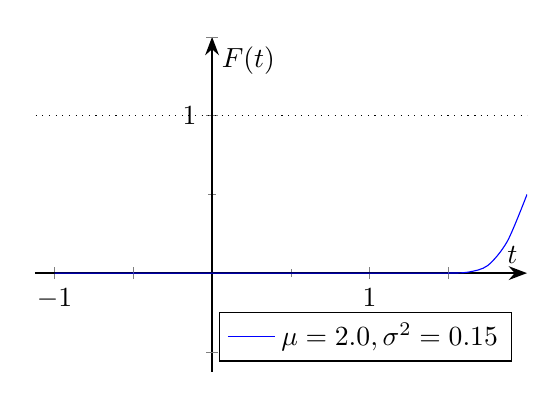
\begin{tikzpicture}
	\pgfmathsetmacro{\countm}{7};
	\pgfmathsetmacro{\counti}{Mod(\theslideIndex-1, \countm)};
	\pgfmathsetmacro{\countj}{(\theslideIndex -1 - \counti)/(\countm)};
	\pgfmathsetmacro{\erwartw}{-1 + 0.5*(\counti)};
	\pgfmathsetmacro{\variance}{0.2 + 0.05*(\countj) };
	\def\Gauss{}
	\begin{axis}[
	legend pos = south east,
	x = 2cm,
	y = 2cm,
	axis lines=middle,
	axis line style={-Stealth,thick},
	xmin=-1.125,xmax=2,ymin=-0.625,ymax=1.5,
	xtick={-1,0,1},
	ytick={0,1},
	extra x ticks={-0.5,1.5},
	extra y ticks={-0.5,1.5},
	extra x tick style={xticklabel=\empty},
	extra y tick style={yticklabel=\empty},
	%xticklabel=\empty,
	%yticklabel=\empty,
	xtick distance=1,
	ytick distance=1,
	xlabel=$t$,
	ylabel=$F(t)$,
	%title={Wonderful plot},
	minor tick num= 1,
	grid style={thin,densely dotted,black!20}]	
	\addplot [name path = B, domain = -1:2, color = blue, smooth] {normcdf(x, \erwartw, \variance};\addlegendentry{$\mu = \erwartw, \sigma^2= \variance$};		
	\addplot [dotted] {1};
	%\path [name path=C] (\pgfkeysvalueof{/pgfplots/xmin},0) -- (\pgfkeysvalueof{/pgfplots/xmax},0);	
	%\addplot [green, fill opacity=0.4] fill between [
	%of=A and C,
	%soft clip={domain=-0.4:0.4},
	%]; 	
	%\addplot [green, fill opacity=0.4] fill between [
	%of=B and C,
	%soft clip={domain=0.75:1.25},
	%]; 
	\end{axis}	
	\end{tikzpicture}\stepcounter{slideIndex}
}

\begin{document}

\chapter{Appendix: Sammlung von Fakten und Beispielen zu Zufallsvariablen}
In diesem Teil des Appendix sammeln wir wesentliche Fakten und Beispiele. Am Ende des Tages ist Stochastik nicht nur abstrakte Ma\ss theorie, ihr m\"usst auch mit Beispielen rumrechnen k\"onnne und ein Gef\"uhl f\"ur Eigenschaften bekommen.\smallskip

Allgemeine Definitionen f\"ur beliebige Zufallsvariablen:
\begin{itemize}
	\item F\"ur eine Zufallsvariable $X$ auf einem Wahrscheinlichkeitsraum $(\Omega, \mathcal A, \mathbb P)$ schreibt man $X\sim F$, falls 
	\begin{align*}
		\mathbb P(X\in (a,b])=\mathbb P_X((a,b])=F(b)-F(a).
	\end{align*}
	Wozu haben wir Ma\ss theorie betrieben? Um die Existenz von stochastischen Modellen (W-Raum und Zufallsvariable) zu beweisen! Wegen Carath\'eodory und der Borel-$\sigma$-Algebra gibt es f\"ur alle Verteilungsfunktionen Zufallsvariablen mit $X\sim F$.
	\item Wenn das Integral existiert, definiert man f\"ur $g:\R\to \overline \R$ messbar $\E[g(X)]=\int_\R g(X(\omega)) \dint \mathbb P(\omega)$ und es gilt aufgrund des Transformationssatzes $\E[g(X)]=\int_\R g(x) \dint \mathbb P_F(x)$. Einige Spezialf\"alle bekommen eigene Namen:
	\begin{itemize}
		\item Erwartungswert f\"ur $g(x)=x$
		\item k.tes Moment f\"ur $g(x)=x^k$
		\item exponentielles Moment f\"ur $g(x)=e^{\lambda x}$ 
	\end{itemize}
	 Wozu haben wir Integrationstheorie betrieben? Um Erwartungswerte und \"ahnliches f\"ur beliebige Zufallsvariablen zu definieren! Ohne Integrationstheorie ginge das nur f\"ur diskrete Zufallsvariablen oder Zufallsvariablen mit Dichten.
	 \end{itemize}


\section{Absolutstetige Zufallsvariablen}
Definitionen und Fakten:
\begin{itemize}
	\item $X\sim F$ hei\ss t absolutstetig, falls $F$ eine Dichte $f$ hat. Es gilt dann $$\mathbb P(X\in (a,b])=\int_a^b f(x)\dint x.$$
	Weil $\{a\}=[a,a]$, gilt  f\"ur absolutstetige Zufallsvariablen $$\mathbb P(X=a)=\int_a^a f(x)dx=0$$ und daher auch 
 	$$ \mathbb P(X\in [a,b])=\mathbb P(X\in (a,b])=\mathbb P(X\in [a,b))=\mathbb P(X\in (a,b)),$$
	es gibt also keine Masse auf einpunktigen Mengen.
	\item Momente lassen sich einfach berechnen. F\"ur messbare $g:\R\to \overline \R$ ist
	\begin{align*}
		\E[g(X)]=\int_\R g(x) f(x) \dint x,
	\end{align*}
	wenn eine der Seiten (und damit die andere) definiert ist.
\end{itemize}

Wichtige Bemerkung f\"ur das Verst\"andniss: Wenn wir irgendeine nichtnegative Funktion $f$ mit $\int_\R f(x)\dint x<\infty$ kennen, so bekommen wir mit $h(x):= C f(x)$ eine Dichte, wobei $\frac 1 C=\int_\R f(x)\dint x$ ist. Unsere Beispiele bestehen also im Prinzip aus den integrierbaren nichtnegativen Funktionen, die wir gut integrieren k\"onnen. Das sind die Exponentialfunktion (gibt die Exponentialverteilung), Exponentialfunktion mit einem Quadrat (gibt die Normalverteilung), Varianten der Funktion $1/x^2$ (gibt die Cauchy Verteilung) oder konstante Funktionen auf kompakten Mengen (gibt die uniformen Verteilungen).

\subsection{Normalverteilung - $\mathcal N(\mu,\sigma^2)$}
Die wichtigste Verteilung der Stochastik ist die Normalverteilung. Das liegt am zentralen Grenzwertsatz. \smallskip

{Vorteile:} 
\begin{itemize}
\item Alle Momente existierten und k\"onnen berechnet werden.
\item Die Verteilungsfunktion ist zwar nicht explizit, dennoch kann vieles ausgerechnet werden.
\item	Zwei Parameter $\mu$ und $\sigma^2$ geben viel Freiheit, die Verteilung an echte Daten anzupassen.
\end{itemize}

{Nachteil:}
\begin{itemize}
	\item Verteilungsfunktion ist nicht explizit gegeben, Wahrscheinlichkeiten der Form $\mathbb P(X\in [a,b])$ m\"ussen daher abgesch\"atzt werden.
\end{itemize}

Wichtige Charakteristiken auf einen Blick:
\begin{center}
\begin{tabular}[h]{|l|l|}
\hline
Parameter& $\mu\in \R$ (Verschiebung), $\sigma^2>0$ (Stauchung)\\
\hline
Wertebereich & $\R$\\
\hline
Verteilungsfunktion & $F_{\mu,\sigma^2}(t)=\int_{-\infty}^t \frac{1}{\sqrt{2\pi \sigma^2}} e^{-\frac{(x-\mu)^2}{2 \sigma^2}} \dint x$ \\
\hline
Dichte & $f_{\mu,\sigma^2}(x)=\frac{1}{\sqrt{2\pi \sigma^2}} e^{-\frac{(x-\mu)^2}{2\sigma^2}}$\\
\hline
Grobe Verteilung der Masse & Viel Masse nah bei $\mu$, extrem wenig bei $+\infty$ und $-\infty$.\\
\hline
Erwartungswert& $\E[X]=\mu$ \\
\hline
Varianz & $\mathbb V[X]=\sigma^2$\\
\hline
Momenterzeugende Funktion& definiert f\"ur alle $t\in\R$, $m_X(t)=e^{\mu t +\frac{\sigma^2 t^2}{2}}$\\
\hline
\end{tabular}

\end{center}
Zum rumspielen hier eine interaktive Graphik. Zu beachten ist: Viel Masse liegt dort, wo die Dichte gro\ss{} ist. Das spiegelt sich dadurch wieder, dass dort die Verteilungsfunktion stark w\"achst. Andersrum: Wenig Masse liegt dort, wo die Verteilungsfunktion flach ist bzw. die Dichte klein ist. 



\subsection{Exponentialverteilung - $\text{Exp}(\lambda)$}

Wichtige Verteilung, besonders in der Anwendungen bei Markovprozessen.\smallskip

{Vorteile:} 
\begin{itemize}
\item Alle Momente existierten und k\"onnen berechnet werden.
\item Verteilungsfunktion und Dichte sind explizit und sehr einfach. Vieles kann berechnet werden.
\end{itemize}

{Nachteil:}
\begin{itemize}
	\item Nur ein Parameter um Verteilung auf Daten anzupassen
\end{itemize}

Wichtige Charakteristiken auf einen Blick:
\begin{center}
\begin{tabular}[h]{|l|l|}
\hline
Parameter& $\lambda>0$ (Stauchung)\\
\hline
Wertebereich & $[0,\infty)$\\
\hline
Verteilungsfunktion & $F_\lambda(t)= (1-e^{-\lambda t})\mathbf 1_{[0,\infty)}(t) $\\
\hline
Dichte & $f_\lambda(x)=\lambda e^{-\lambda x} \mathbf 1_{[0,\infty)}(x)$\\
\hline
Grobe Verteilung der Masse & Viel Masse nah bei $0$, wenig bei $+\infty$\\
\hline
Erwartungswert& $\E[X]=\frac{1}{\lambda}$ \\
\hline
Varianz & $\mathbb V[X]=\frac{1}{\lambda^2} $\\
\hline
Momenterzeugende Funktion& definiert f\"ur alle $t<\lambda$, $m_X(t)=\frac{\lambda}{\lambda-t}$\\
\hline
\end{tabular}

\end{center}


\subsection{Uniforme Verteilung - $\mathcal U([a,b])$}

Modell f\"ur das einfachste Experiment, Ziehen aus einem Intervall ohne Bevorzugung verschiedener Bereiche.\smallskip

{Vorteile:} 
\begin{itemize}
\item Alle Momente existierten und k\"onnen berechnet werden.
\item Verteilungsfunktion und Dichte sind explizit und sehr einfach. Vieles kann berechnet werden.
\item Man kann alle anderen Verteilungen aus $\mathcal U([0,1])$ gewinnen, theoretisch reicht also die uniforme Verteilung f\"ur alles aus!
\end{itemize}

{Nachteile:}
\begin{itemize}
	\item Gar kein Parameter um Verteilung auf Daten anzupassen
	\item Eher langweilig.
\end{itemize}

Wichtige Charakteristiken auf einen Blick:
\begin{center}
\begin{tabular}[h]{|l|l|}
\hline
Parameter& keine Parameter \\
\hline
Wertebereich & $[a,b]$\\
\hline
Verteilungsfunktion & $F(t)= \frac{t-a}{b-a}1_{[a,b]}(t)+1_{[b,\infty)}(t) $\\
\hline
Dichte & $f(x)= \frac{1}{b-a}1_{[a,b]}(x)$\\
\hline
Grobe Verteilung der Masse & uniform auf $[a,b]$ (daher der Name)\\
\hline
Erwartungswert& $\E[X]=\frac{a+b}{2}$ \\
\hline
Varianz & $\mathbb V[X]=\frac{(b-a)^2}{12}$\\
\hline
Momenterzeugende Funktion& definiert f\"ur alle $t\in \R$, $m_X(t)=\begin{cases} \frac{e^{bt}-e^{at}}{(b-a)t}&:t\neq 0\\ 1&:t=0 \end{cases}$\\
\hline
\end{tabular}

\end{center}


\subsection{Gammaverteilung - $\Gamma(\alpha,\beta)$}


{Vorteile:} 
\begin{itemize}
\item Sehr flexibel durch zwei Parameter, erlaubt Modellierung sehr unterschiedlicher Masseverteilungen mit einem Modell. Ein Parameter beschreibt Verhalten bei $0$, einer bei $+\infty$
\item Exponentialverteilung ist Spezialfall: $\text{Exp}(\lambda)=\Gamma(1,\lambda)$
\item Alle Momente existierten und k\"onnen berechnet werden, Momenterzeugende Funktion kann problemlos abgeleitet werden.
\item Viel kann berechnet werden.
\end{itemize}

{Nachteil:}
\begin{itemize}
	\item Verteilungsfunktion nicht explizit.
\end{itemize}

Wichtige Charakteristiken auf einen Blick:
\begin{center}
\begin{tabular}[h]{|l|l|}
\hline
Parameter& $\alpha>0$, (Masse bei $0$) $\beta>0$ (Masse bei $+\infty$)\\
\hline
Wertebereich & $(0,\infty)$\\
\hline
Verteilungsfunktion & nicht explizit\\
\hline
Dichte & $f_{\alpha,\beta}(x)= 1_{(0,\infty)}(x) \frac{\beta^\alpha}{\Gamma(\alpha)} x^{\alpha-1} e^{-\beta x}$\\
\hline
Grobe Verteilung der Masse & wenig Masse bei $+\infty$ (Dichte f\"allt exp.)\\
& viel Masse bei $0$ f\"ur $p<1$, wenig f\"ur $p>0$\\
\hline
Erwartungswert& $\E[X]=\frac{\alpha}{\beta}$ \\
\hline
Varianz & $\mathbb V[X]=\frac{\alpha}{\beta^2}$\\
\hline
Momenterzeugende Funktion& definiert f\"ur $t<\beta$, $m_X(t)=(\beta/(\beta-t))^\alpha$\\
\hline
\end{tabular}
\end{center}


\subsection{Cauchy Verteilung - $\text{Cauchy}(s,t)$}
Die Cauchy-Verteilung ist eine sogenannte \glqq heavz-tailed\grqq{} Verteilung, d. h. viel Masse liegt bei unendlich. F\"ur uns hat die Verteilung eigentlich nur Nachteile, es geht so ziemlich alles schief.

{Vorteile:} 
\begin{itemize}
\item	Zwei Parameter $s$ und $t$ geben viel Freiheit, die Verteilung an echte Daten anzupassen. 
\item Verteilungsfunktion und Dichte sind explizit. 
\end{itemize}

{Nachteile}
\begin{itemize}
	\item Klassisches Beispiel f\"ur eine Verteilung, deren Erwartungswert nicht wohldefiniert ist.
\end{itemize}

Wichtige Charakteristiken auf einen Blick:
\begin{center}
\begin{tabular}[h]{|l|l|}
\hline
Parameter& $t\in \R$ (Verschiebung), $s>0$ (Stauchung)\\
\hline
Wertebereich & $\R$\\
\hline
Verteilungsfunktion & $F_{s,t}(r)= \frac{1}{2}+\frac{1}{\pi} \arctan(\frac{r-t}{s})$\\
\hline
Dichte & $f_{s,t} (x)=\frac{1}{\pi}\frac{s}{s^2+(x-t)^2}$\\
\hline
Grobe Verteilung der Masse & viel Masse bei $0$, aber auch viel bei $+\infty$ und $-\infty$\\
\hline
Erwartungswert& nicht wohldefiniert! \\
\hline
Varianz & existiert nicht!\\
\hline
Momenterzeugende Funktion& f\"ur kein $t\in\R$ definiert\\
\hline
\end{tabular}
\end{center}




\section{Diskrete Zufallsvariablen}
Definitionen und Fakten:
\begin{itemize}
	\item $X\sim F$ hei\ss t diskret, falls $F$ eine diskrete Verteilungsfunktion ist (d. h. $F$ ist st\"uckweise konstant mit Spr\"ungen $p_i$ an Stellen $a_i$). Man kann dann immer $$F(t)=\sum_{k=1}^N p_k \mathbf 1_{[a_k,\infty)}(t),\quad t\in\R,$$ schreiben, wobei $N\in \N\cup \{+\infty\}$, $a_i\in\R$ f\"ur $i=1,...,N$ und $\sum_{k=1}^N p_k=1$. Wir kennen in dem Fall diskreter Verteilungen auch das Ma\ss{} $\mathbb P_F$ expliziert, es gilt
	$$\mathbb P_F=\sum_{k=1}^N p_k \delta_{a_k},$$ f\"ur alle $A\in \mathcal B(\R)$. Weil per Definition $\mathbb P(X\in A)=\mathbb P_F(A)$, folgt damit
	 $$\mathbb P(X\in A)=\mathbb P_F(A)=\sum_{k=1, a_k\in A}^N p_k\quad \text{ und insbesondere }\quad \mathbb P(X=a_k)=p_k.$$
	Wir sehen also, dass $X$ ausschlie\ss lich die Werte $a_1,...,a_N$ mit positiver Wahrscheinlichkeit annimmt, denn es gilt
	$$\mathbb P(X\notin \{a_1,...,a_n\})=1-\mathbb P(X\in \{a_1,...,a_N\})=1-1=0.$$	
	Wir nennen die $p_k$ Wahrscheinlichkeiten von $a_k$, manchmal auch Wahrscheinlichkeitsgewichte. Im Gegensatz zu absolutstetigen Zufallsvariablen haben diskrete Zufallsvariablen also durchaus Masse auf einpunktigen Mengen, n\"ahmlich gerade auf den Mengen $\{a_1\}, ...$.
	\item Momente lassen sich einfach berechnen. F\"ur messbare $g:\R\to \overline \R$ ist
	\begin{align*}
		\E[g(X)]=\sum_{k=1}^N p_k g(a_k),
	\end{align*}
	wenn eine der Seiten (und damit die andere) definiert ist.
\end{itemize}
Wie bei absolutstetigen Verteilungen k\"onnen wir uns aus den Analysis 1 Kenntnissen im Prinzip alle klassischen diskreten Verteilungen erraten. Es gibt zwei wesentliche F\"alle:
\begin{itemize}
	\item $N<\infty$: Man w\"ahle irgendwelche $a_1,...,a_N\in\R$ und denke sich irgendwelche $p_1,...,p_N \geq 0$ aus, die sich zu $1$ addieren.
	\item $N=+\infty$: Man w\"ahle irgendeine Folge $a_1,a_2,...\in \R$ und benutze eine bekannte konvergente Reihe $\sum_{k=1}^\infty b_k$ aus Analysis 1. Ist $\frac 1 C=\sum_{k=1}^\infty b_k$, so setzt man $p_k=Cb_k$. Schon haben wir eine diskrete Verteilung! Wenn wir jetzt an Analysis 1 denken, fallen uns nur wenige konvergente Reihen mit positiven Summanden ein. Das ist die 
	sche Reihe (gibt die geometrische Verteilung) und die die Exponentialreihe (gibt die Poisson Verteilung). Das war es eigentlich schon.
\end{itemize}



\subsection{Bernoulli Verteilung - $\text{Ber}(p)$}

{Vorteile:} 
\begin{itemize}
	\item Total einfach, Modell f\"ur den M\"unzwurf einer unfairen M\"unze.
	\item Alles, wirklich alles, l\"asst sich sofort ausrechnen.
\end{itemize}

{Nachteil:}
\begin{itemize}
	\item Komplett langweilig!
\end{itemize}

Wichtige Charakteristiken auf einen Blick:
\begin{center}
\begin{tabular}[h]{|l|l|}
\hline
Parameter& $p\in [0,1]$ \\
\hline
Wertebereich & $0$ oder $1$\\
\hline
Wahrscheinlichkeitsgewichte& $p_1=p, p_0=q$ wobei $q=1-p$\\
\hline
Grobe Verteilung der Masse & Anteil $p$ der Masse auf der $1$, Rest auf der $0$\\
\hline
Erwartungswert& $\E[X]=p$ \\
\hline
Varianz & $\mathbb V[X]=pq$\\
\hline
Momenterzeugende Funktion& definiert f\"ur alle $t\in \R$, $m_X(t)=1-t+pe^t$\\
\hline
\end{tabular}
\end{center}





\subsection{Binomial Verteilung - $\text{Bin}(n,p)$}

{Vorteil:} 
\begin{itemize}
	\item Modell f\"ur Ziehen mit Zur\"ucklegen, klare Interpretation ($p_k$ ist die Wahrscheinlichkeit, bei $n$ Versuchen, $k$ Treffer zu landen).
	\item Viele Formeln berechenbar. Es gibt einen einfachen Beweis f\"ur den zentralen Grenzwertsatz.
\end{itemize}
Nachteil:
\begin{itemize}
 	\item Teilweise fuzzelig zum Rechnen. Muss immer irgendwie die Binomialformel ins Spiel bringen.
\end{itemize}
Wichtige Charakteristiken auf einen Blick:
\begin{center}
\begin{tabular}[h]{|l|l|}
\hline
Parameter& $n\in \N, p\in [0,1]$ \\
\hline
Wertebereich & $\{0,...,n\}$\\
\hline
Wahrscheinlichkeitsgewichte& $p_k=\left(n\atop k\right) p^k(1-p)^{n-k}$\\
\hline
Grobe Verteilung der Masse & viel Masse in der Mitte von $\{0,...,n\}$, wenig bei $0$ und $n$\\
\hline
Erwartungswert& $\E[X]=np $ \\
\hline
Varianz & $\mathbb V[X]=npq$\\
\hline
Momenterzeugende Funktion& definiert f\"ur alle $t\in \R$, $m_X(t)=(pe^t+1-p)^n$\\
\hline
\end{tabular}
\end{center}


\subsection{Poisson Verteilung $\text{Poi}(\lambda)$}

{Vorteile:} 
\begin{itemize}
	\item Viele Formeln berechenbar, ist auch eine gute Reihe!
\end{itemize}


Wichtige Charakteristiken auf einen Blick:
\begin{center}
\begin{tabular}[h]{|l|l|}
\hline
Parameter& $\lambda>0$ \\
\hline
Wertebereich & $\N_0$\\
\hline
Wahrscheinlichkeitsgewichte& $p_k=e^{-\lambda} \frac{\lambda^k}{k!}$\\
\hline
Grobe Verteilung der Masse & viel Masse auf kleinen Zahlen, wenig bei $+\infty$.\\
\hline
Erwartungswert& $\E[X]=\lambda$ \\
\hline
Varianz & $\mathbb V[X]=\lambda$\\
\hline
Momenterzeugende Funktion& definiert f\"ur alle $t\in \R$, $m_X(t)=\exp(\lambda(e^t-1))$\\
\hline
\end{tabular}
\end{center}



\subsection{Geometrische Verteilung $\text{Geo}(p)$}

{Vorteile:} 
\begin{itemize}
	\item Viele Formeln berechenbar, ist auch eine gute Reihe!
\end{itemize}

Nachteil:
\begin{itemize}
	\item Teilweise fuzzelig zum Rechnen. Viel Indexverschiebung als analog zur Substitution im Fall der Dichten.
\end{itemize}


Wichtige Charakteristiken auf einen Blick:
\begin{center}
\begin{tabular}[h]{|l|l|}
\hline
Parameter& $p>0$ \\
\hline
Wertebereich & $\N\backslash \{0\}$\\
\hline
Wahrscheinlichkeitsgewichte& $p_k=p(1-p)^{n-1}$\\
\hline
Grobe Verteilung der Masse & viel Masse auf kleinen Zahlen, wenig bei $+\infty$.\\
\hline
Erwartungswert& $\E[X]=\frac 1 p$ \\
\hline
Varianz & $\mathbb V[X]=\frac{1-p}{p^2}$\\
\hline
Momenterzeugende Funktion& definiert f\"ur alle $t\in \R$, $m_X(t)=\frac{pe^t}{1-(1-p)e^t}$\\
\hline
\end{tabular}
\end{center}

\end{document}

